\documentclass[tikz, border=10pt]{standalone}
\usepackage{amsmath}


% 1. Use the standard Computer Modern Sans Serif
\usepackage[T1]{fontenc}
\renewcommand{\familydefault}{\sfdefault}


\begin{document}
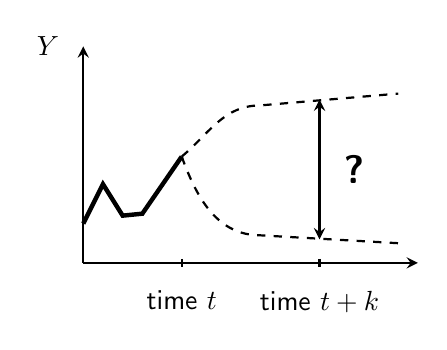
\begin{tikzpicture}[>=stealth, scale = 0.5]

    % --- Coordinates ---
    % Historical/Observed Data points
    \coordinate (p0) at (0, 0.5);
    \coordinate (p1) at (0.5, 1.5);
    \coordinate (p2) at (1.0, 0.7);
    \coordinate (p3) at (1.5, 0.75);
    \coordinate (p4) at (2.5, 2.2); % Point at time t

    % --- X-Axis ---
    \draw[->, thick] (0, -0.5) -- (8.5, -0.5);
    \draw[->, thick] (0, -0.5) -- (0., 5) node[left=5pt] {$Y$};
    
    % Ticks and Labels for X-axis
    \draw[thick] (2.5, -0.4) -- (2.5, -0.6) node[below=5pt] {time $t$};
    \draw[thick] (6.0, -0.4) -- (6.0, -0.6) node[below=5pt] {time $t+k$};

    % --- Observed Data (Solid Line) ---
    \draw[ultra thick] (p0) -- (p1) -- (p2) -- (p3) -- (p4);

    % --- Forecast/Uncertainty (Dashed Lines) ---
    % Upper Bound
    \draw[dashed, thick] (p4) to[out=40, in=180] (4.5, 3.5) -- (8, 3.8);
    
    % Lower Bound
    \draw[dashed, thick] (p4) to[out=-70, in=180] (4.5, 0.2) -- (8, 0.0);

    % --- Uncertainty Arrow and Question Mark ---
    \draw[<->, thick] (6, 3.65) -- (6, 0.1) node[midway, right=5pt] {\Large \textbf{?}};

\end{tikzpicture}
\end{document}